\documentclass[12pt,letterpaper]{article}
\usepackage{graphicx,textcomp}
\usepackage{caption}
\usepackage{natbib}
\usepackage{setspace}
\usepackage{fullpage}
\usepackage{color}
\usepackage[reqno]{amsmath}
\usepackage{amsthm}
\usepackage{fancyvrb}
\usepackage{amssymb,enumerate}
\usepackage[all]{xy}
\usepackage{endnotes}
\usepackage{lscape}
\newtheorem{com}{Comment}
\usepackage{float}
\usepackage{hyperref}
\newtheorem{lem} {Lemma}
\newtheorem{prop}{Proposition}
\newtheorem{thm}{Theorem}
\newtheorem{defn}{Definition}
\newtheorem{cor}{Corollary}
\newtheorem{obs}{Observation}
\usepackage[compact]{titlesec}
\usepackage{dcolumn}
\usepackage{tikz}
\usetikzlibrary{arrows}
\usepackage{multirow}
\usepackage{xcolor}
\newcolumntype{.}{D{.}{.}{-1}}
\newcolumntype{d}[1]{D{.}{.}{#1}}
\definecolor{light-gray}{gray}{0.65}
\usepackage{url}
\usepackage{listings}
\usepackage{color}

\definecolor{codegreen}{rgb}{0,0.6,0}
\definecolor{codegray}{rgb}{0.5,0.5,0.5}
\definecolor{codepurple}{rgb}{0.58,0,0.82}
\definecolor{backcolour}{rgb}{0.95,0.95,0.92}

\lstdefinestyle{mystyle}{
	backgroundcolor=\color{backcolour},   
	commentstyle=\color{codegreen},
	keywordstyle=\color{magenta},
	numberstyle=\tiny\color{codegray},
	stringstyle=\color{codepurple},
	basicstyle=\footnotesize,
	breakatwhitespace=false,         
	breaklines=true,                 
	captionpos=b,                    
	keepspaces=true,                 
	numbers=left,                    
	numbersep=5pt,                  
	showspaces=false,                
	showstringspaces=false,
	showtabs=false,                  
	tabsize=2
}
\lstset{style=mystyle}
\newcommand{\Sref}[1]{Section~\ref{#1}}
\newtheorem{hyp}{Hypothesis}

\title{Problem Set 3}
\date{Due: November 19, 2022}
\author{Applied Stats/Quant Methods 1}


\begin{document}
	\maketitle
	\section*{Instructions}
	\begin{itemize}
		\item Please show your work! You may lose points by simply writing in the answer. If the problem requires you to execute commands in \texttt{R}, please include the code you used to get your answers. Please also include the \texttt{.R} file that contains your code. If you are not sure if work needs to be shown for a particular problem, please ask.
	\item Your homework should be submitted electronically on GitHub.
	\item This problem set is due before 23:59 on Sunday November 19, 2023. No late assignments will be accepted.

	\end{itemize}
	
\noindent In this problem set, you will run several regressions and create an add variable plot (see the lecture slides) in \texttt{R} using the \texttt{incumbents\_subset.csv} dataset. Include all of your code.

\section*{Question 1}
\vspace{.25cm}
\noindent We are interested in knowing how the difference in campaign spending between incumbent and challenger affects the incumbent's vote share. 
	\begin{enumerate}
		\item Run a regression where the outcome variable is \texttt{voteshare} and the explanatory variable is \texttt{difflog}.
		
		At the beginning, I imported the data set, familiarised myself with it, and then extracted relevant data for the Questions and confirmed that the remaining data frame \texttt{df} contained the correct data.
		
			\lstinputlisting[language=R, firstline=41, lastline=56]{PS3.R}
		
		\texttt I note that I do not have the code book for the data set, and so do not know the real units for each variable. Therefore, my answers will refer to changes in "unit points" for accuracy.
		
			\lstinputlisting[language=R, firstline=64, lastline=66]{PS3.R}
		
		\begin{table}[!htbp]
			\centering
			\captionsetup{justification=centering, font = footnotesize}
			\caption{Linear Regression Results: Positive Correlation\\
				between Vote Share of Incumbent\\
				and Difference in Campaign Spending} 
			\label{} 
			\begin{tabular}{@{\extracolsep{5pt}}lD{.}{.}{-3} } 
				\\[-1.8ex]\hline 
				\hline \\[-1.8ex] 
				& \multicolumn{1}{c}{\textit{Dependent variable:}} \\ 
				\cline{2-2} 
				\\[-1.8ex] & \multicolumn{1}{c}{voteshare} \\ 
				\hline \\[-1.8ex] 
				difflog & 0.042^{***} \\ 
				& (0.001) \\ 
				& \\ 
				Constant & 0.579^{***} \\ 
				& (0.002) \\ 
				& \\ 
				\hline \\[-1.8ex] 
				Observations & \multicolumn{1}{c}{3,193} \\ 
				R$^{2}$ & \multicolumn{1}{c}{0.367} \\ 
				Adjusted R$^{2}$ & \multicolumn{1}{c}{0.367} \\ 
				Residual Std. Error & \multicolumn{1}{c}{0.079 (df = 3191)} \\ 
				F Statistic & \multicolumn{1}{c}{1,852.791$^{***}$ (df = 1; 3191)} \\ 
				\hline 
				\hline \\[-1.8ex] 
				\textit{Note:}  & \multicolumn{1}{r}{$^{*}$p$<$0.1; $^{**}$p$<$0.05; $^{***}$p$<$0.01} \\ 
			\end{tabular} 
		\end{table}
		
		\texttt This bi-variate linear regression model indicates that for \textbf{every 1-unit increase} in the difference in campaign spending between the incumbent and challenger, on average, the vote share for the incumbent increases by \textbf{approx. 0.04 unit points}.
		
		The coefficient has a p-value less than 0.001, which is less than a critical value of 0.05, giving evidence to reject the null hypothesis that the relationship between difference in campaign spending and incumbent vote share is zero - and giving evidence for the alternative hypothesis that the relationship is non-zero. It is not possible to indicate a causal relationship with this method.
		
		\item Make a scatterplot of the two variables and add the regression line.
		
			\lstinputlisting[language=R, firstline=74, lastline=92]{PS3.R}
		
			\begin{figure}[H]
				\centering
				\captionsetup{justification=centering, font = footnotesize}
				\caption{Scatterplot and Regression Line: Positive Correlation\\
					between Vote Share of Incumbent and Difference in Campaign Spending.}
				\label{fig:plot_Q1}
				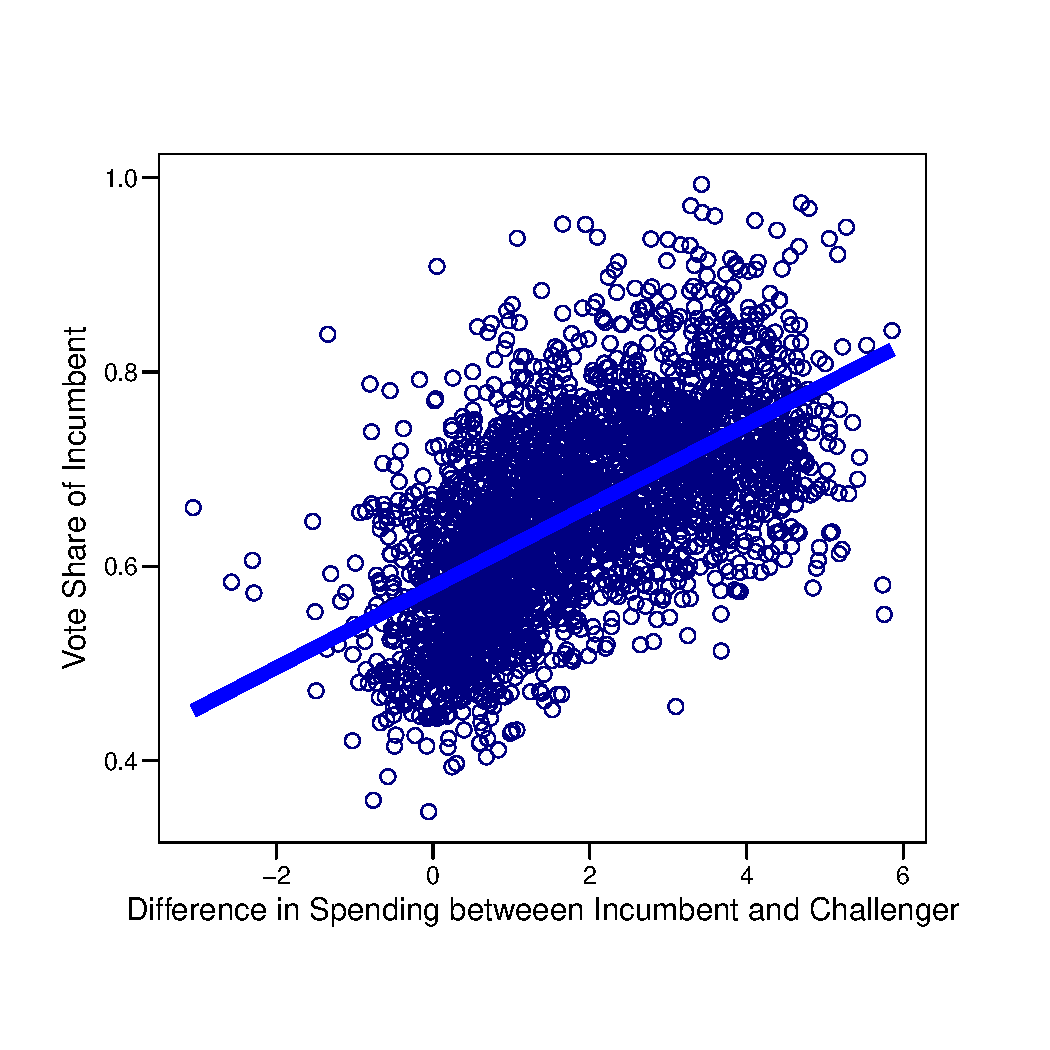
\includegraphics[width=.75\textwidth, trim = 0 2cm 0 2cm, clip]{plot_Q1.pdf}
			\end{figure}
		
		\item Save the residuals of the model in a separate object.
		
				\lstinputlisting[language=R, firstline=96, lastline=101]{PS3.R}
		
		\item Write the prediction equation.
		
			\texttt Below is a generic formal prediction equation  for a bi-variate linear regression model:
		
		\begin{align*}
			Y_i &= \beta_0 + \beta_1 X_i + \varepsilon
		\end{align*}
		
		\texttt The components are:
		\begin{enumerate}
			\item $Y$: The (predicted) value for the outcome variable
			\item $\beta_0$: The y-intercept (i.e. when the explanatory variable equals zero).
			\item $\beta_1$: The coefficient or slope. This represents the \textbf{average change} in $Y$ with a one-unit change in the corresponding explanatory variable.
			\item  $X_i$: The value for the (input) explanatory variable.
			\item $\varepsilon$: The \textbf{theoretical} (stochastic) error term, which represents the unobserved/unaccounted for factors which influence $Y$ yet are not included in the model.
			
			Note a key assumption for linear regression models is that $\varepsilon$ has a \textit{constant and independent average effect} on one or several variables within the model which cancels itself out when given a large sample N (see notation below). Given this theoretical assumption, it is typically excluded from written prediction equations. This is why a prediction equation is also called the "least-square equation".
			
				$$\varepsilon_i \stackrel{iid}{\sim} N(O, \sigma^2)$$
			
			Also note that the theoretical error $\varepsilon$ is distinct from the observed residual $e_i$ for each data point. Residuals are discussed in greater detail in Question 4.
			
		\end{enumerate}
		
		\texttt Below is the prediction equation for the linear regression where the outcome variable is \texttt{voteshare} and the explanatory variable is \texttt{difflog}.
		
		\begin{align*}
			&\text{Predicted vote share for the incumbent} = \\ &\beta_\text{vote share for the incumbent when spending difference is zero} \\ &+ (\beta_\text{coefficient for 1-unit increase in spending difference} \times X_\text{spending difference})
		\end{align*}
		
		\texttt Below is the prediction equation with the relevant values (rounded to two decimal places):
		\begin{align*}
			\text{Predicted vote share for the incumbent} = 0.58 + (0.04 * X_\text{spending difference})
		\end{align*}
	
		\texttt This equation can be used to find the predicted (estimated) vote share for the incumbent, corresponding to the input value for the spending difference between the incumbent and challenger.
		
		Caution should be maintained for inputting values of spending difference which are \textbf{greater than 5.86 and lower than -3.06}. These are the maximum and minimum observed data points for spending difference, and so the model cannot be assumed to be valid outside of these value thresholds.
		
			\lstinputlisting[language=R, firstline=110, lastline=111]{PS3.R}
	
	\end{enumerate}
	
	
\newpage
\section*{Question 2}
\noindent We are interested in knowing how the difference between incumbent and challenger's spending and the vote share of the presidential candidate of the incumbent's party are related.	\vspace{.25cm}
	\begin{enumerate}
		\item Run a regression where the outcome variable is \texttt{presvote} and the explanatory variable is \texttt{difflog}.
		
			\lstinputlisting[language=R, firstline=121, lastline=123]{PS3.R}
			
			\begin{table}[!htbp]
				\centering
				\captionsetup{justification=centering, font = footnotesize}
				\caption{Linear Regression Results: Positive Correlation\\
					between Vote Share of Presidential Candidate of Incumbent's Party\\
					and Difference in Campaign Spending} 
				\label{} 
				\begin{tabular}{@{\extracolsep{5pt}}lD{.}{.}{-3} } 
					\\[-1.8ex]\hline 
					\hline \\[-1.8ex] 
					& \multicolumn{1}{c}{\textit{Dependent variable:}} \\ 
					\cline{2-2} 
					\\[-1.8ex] & \multicolumn{1}{c}{presvote} \\ 
					\hline \\[-1.8ex] 
					difflog & 0.024^{***} \\ 
					& (0.001) \\ 
					& \\ 
					Constant & 0.508^{***} \\ 
					& (0.003) \\ 
					& \\ 
					\hline \\[-1.8ex] 
					Observations & \multicolumn{1}{c}{3,193} \\ 
					R$^{2}$ & \multicolumn{1}{c}{0.088} \\ 
					Adjusted R$^{2}$ & \multicolumn{1}{c}{0.088} \\ 
					Residual Std. Error & \multicolumn{1}{c}{0.110 (df = 3191)} \\ 
					F Statistic & \multicolumn{1}{c}{307.715$^{***}$ (df = 1; 3191)} \\ 
					\hline 
					\hline \\[-1.8ex] 
					\textit{Note:}  & \multicolumn{1}{r}{$^{*}$p$<$0.1; $^{**}$p$<$0.05; $^{***}$p$<$0.01} \\ 
				\end{tabular} 
			\end{table} 
			
			\texttt This bi-variate linear regression model indicates that for \textbf{every 1-unit increase} in the difference in campaign spending between the incumbent and challenger, on average, the vote share for the Presidential Candidate of the Incumbent's Party increases by \textbf{approx. 0.02 unit points}.
			
			The coefficient has a p-value less than 0.001, which is less than a critical value of 0.05, giving evidence to reject the null hypothesis that the relationship between difference in campaign spending and vote share of the Incumbent Party's Presidential Candidate is zero - and giving evidence for the alternative hypothesis that the relationship is non-zero. It is not possible to indicate a causal relationship with this method.
		
		\item Make a scatterplot of the two variables and add the regression line.
		
			\lstinputlisting[language=R, firstline=137, lastline=155]{PS3.R}
		
			\begin{figure}[H]
				\centering
				\captionsetup{justification=centering, font = footnotesize}
				\caption{Scatterplot and Regression Line: Positive Correlation\\
					between Vote Share of Presidential Candidate of Incumbent's Party\\
					and Difference in Campaign Spending.}
				\label{fig:plot_Q2}
				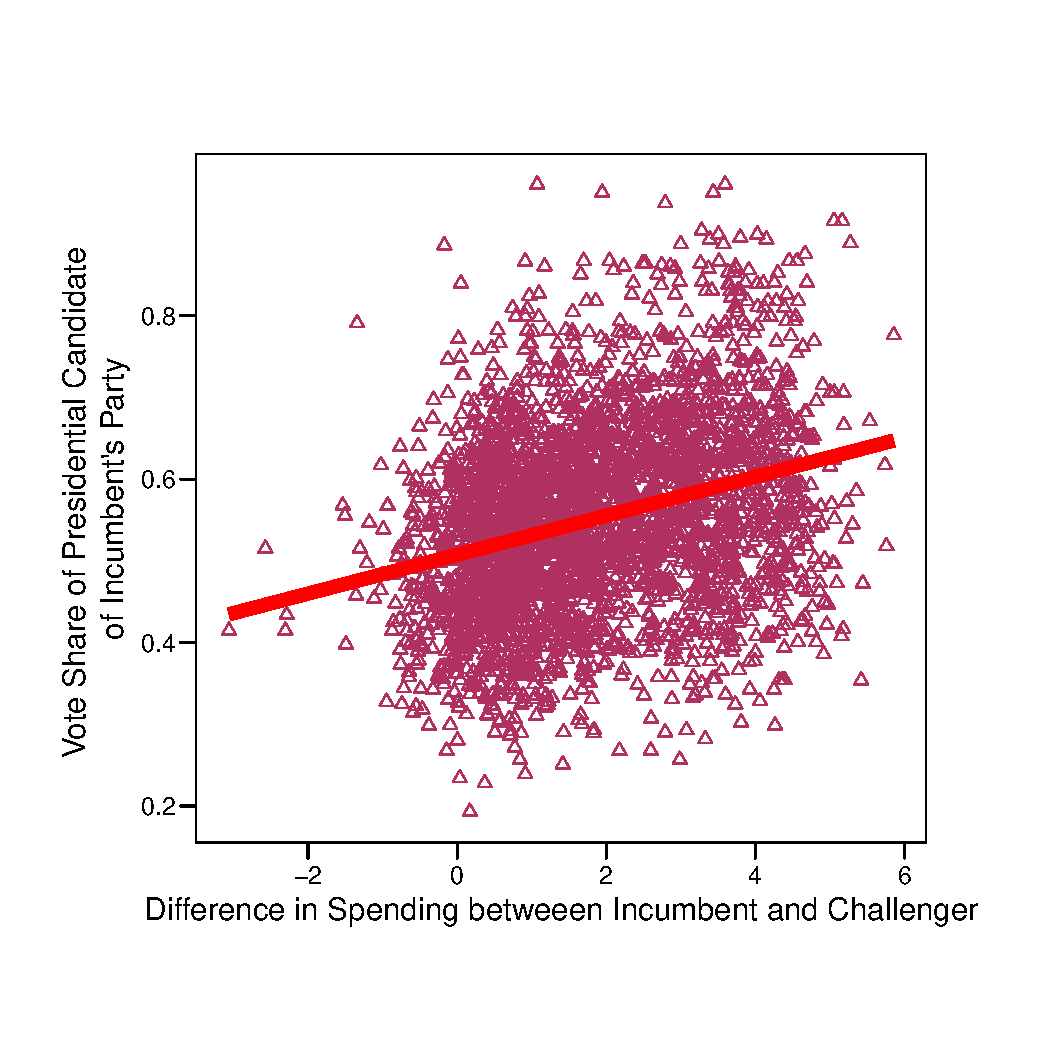
\includegraphics[width=.75\textwidth, trim = 0 2cm 0 2cm, clip]{plot_Q2.pdf}
			\end{figure}
		
		\item Save the residuals of the model in a separate object.
		
			\lstinputlisting[language=R, firstline=159, lastline=164]{PS3.R}
		
		\item Write the prediction equation.
		
			\texttt Below is the prediction equation for the linear regression where the outcome variable is \texttt{presvote} and the explanatory variable is \texttt{difflog}. See Question 1 for generalised discussion.
		
		\begin{align*}
			&\text{Predicted vote share for the incumbent party's presidential candidate} = \\ &\beta_\text{vote share for the incumbent party's presidential candidate when spending difference is zero} \\ &+ \beta_\text{coefficient for 1-unit increase in spending difference} X_\text{spending difference}
		\end{align*}
		
		\texttt Below is the prediction equation with the relevant values (rounded to two decimal places):
		\begin{align*}
			&\text{Predicted vote share for the incumbent party's presidential candidate} = \\ & 0.51 + (0.02 * X_\text{spending difference})
		\end{align*}
		
		\texttt This equation can be used to find the predicted (estimated) vote share for the incumbent party's presidential candidate, corresponding to the input value for the spending difference between the incumbent and challenger.
		
		Caution should be maintained for inputting values of spending difference which are \textbf{greater than 5.86 and lower than -3.06}. These are the maximum and minimum observed data points for spending difference, and so the model cannot be assumed to be valid outside of these value thresholds. See Question 1, Part 4 for code checking min/max value.
		
	\end{enumerate}
	
\newpage	
\section*{Question 3}
\noindent We are interested in knowing how the vote share of the presidential candidate of the incumbent's party is associated with the incumbent's electoral success.
	\vspace{.25cm}
	\begin{enumerate}
		\item Run a regression where the outcome variable is \texttt{voteshare} and the explanatory variable is \texttt{presvote}.

			\lstinputlisting[language=R, firstline=181, lastline=183]{PS3.R}
			
			\begin{table}[!htbp]
				\centering 
				\captionsetup{justification=centering, font = footnotesize}
				\caption{Linear Regression Results: Positive Correlation\\
					between Vote Share of Presidential Candidate of Incumbent's Party\\
					and Vote Share of Incumbent} 
				\label{} 
				\begin{tabular}{@{\extracolsep{5pt}}lD{.}{.}{-3} } 
					\\[-1.8ex]\hline 
					\hline \\[-1.8ex] 
					& \multicolumn{1}{c}{\textit{Dependent variable:}} \\ 
					\cline{2-2} 
					\\[-1.8ex] & \multicolumn{1}{c}{voteshare} \\ 
					\hline \\[-1.8ex] 
					presvote & 0.388^{***} \\ 
					& (0.013) \\ 
					& \\ 
					Constant & 0.441^{***} \\ 
					& (0.008) \\ 
					& \\ 
					\hline \\[-1.8ex] 
					Observations & \multicolumn{1}{c}{3,193} \\ 
					R$^{2}$ & \multicolumn{1}{c}{0.206} \\ 
					Adjusted R$^{2}$ & \multicolumn{1}{c}{0.206} \\ 
					Residual Std. Error & \multicolumn{1}{c}{0.088 (df = 3191)} \\ 
					F Statistic & \multicolumn{1}{c}{826.950$^{***}$ (df = 1; 3191)} \\ 
					\hline 
					\hline \\[-1.8ex] 
					\textit{Note:}  & \multicolumn{1}{r}{$^{*}$p$<$0.1; $^{**}$p$<$0.05; $^{***}$p$<$0.01} \\ 
				\end{tabular} 
			\end{table} 

			\texttt This bi-variate linear regression model indicates that for \textbf{every 1-unit increase} in the Vote Share of the Presidential Candidate of the Incumbent's Party, on average, the Vote Share for the Incumbent increases by \textbf{approx. 0.39 unit points}.
			
			The coefficient has a p-value less than 0.001, which is less than a critical value of 0.05, giving evidence to reject the null hypothesis that the relationship between the vote share of the Incumbent Party's Presidential Candidate and the vote share of the Incumbent is zero - and giving evidence for the alternative hypothesis that the relationship is non-zero. It is not possible to indicate a causal relationship with this method.

		\item Make a scatterplot of the two variables and add the regression line. 
		
			\lstinputlisting[language=R, firstline=197, lastline=215]{PS3.R}
		
			\begin{figure}[H]
				\centering
				\captionsetup{justification=centering, font = footnotesize}
				\caption{Scatterplot and Regression Line: \\
					Positive Correlation between Vote Share of Presidential Candidate of Incumbent's Party \\
					and Vote Share of Incumbent.}
				\label{fig:plot_Q3}
				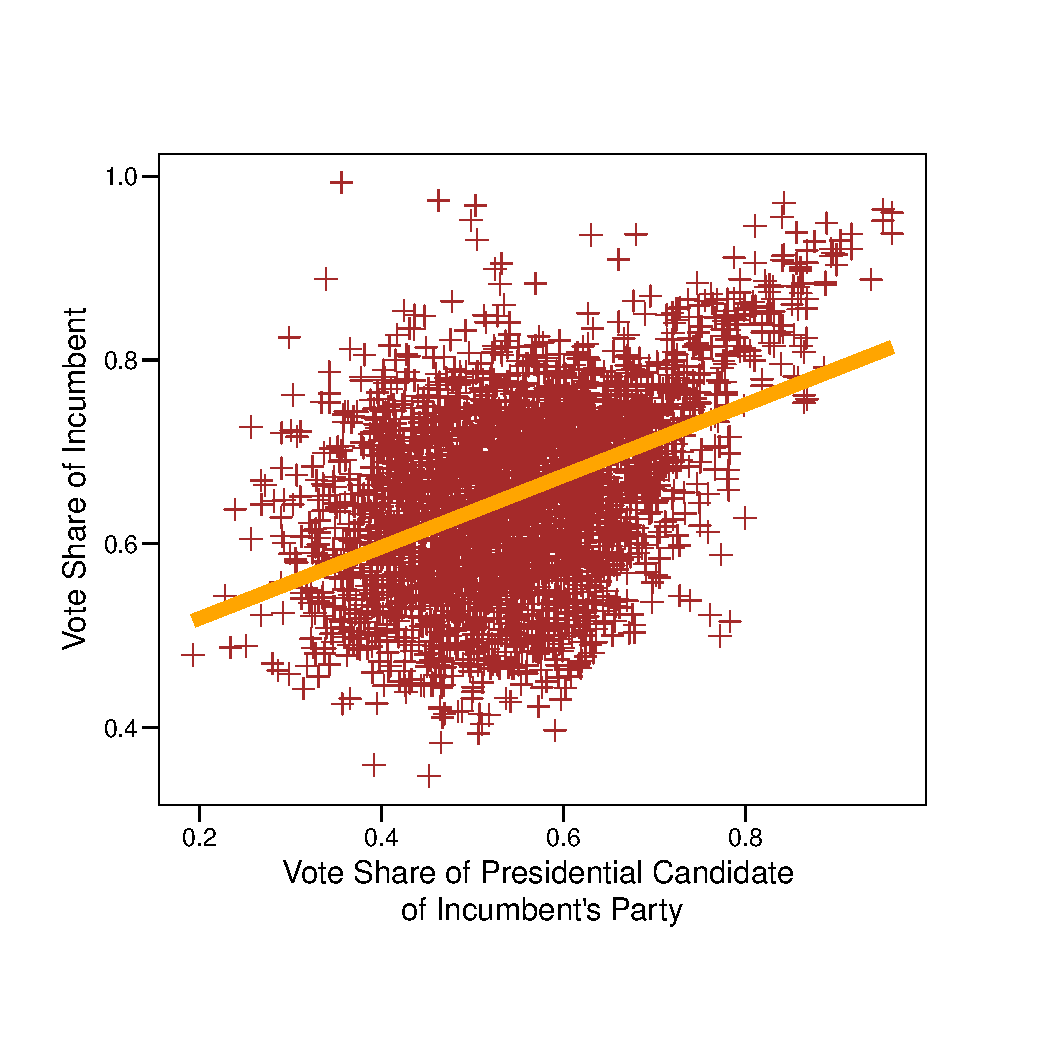
\includegraphics[width=.75\textwidth, trim = 0 2cm 0 2cm, clip]{plot_Q3.pdf}
			\end{figure}
		
		\item Write the prediction equation.
		
			\texttt Below is the prediction equation for the linear regression where the outcome variable is \texttt{voteshare} and the explanatory variable is \texttt{presvote}. See Question 1 for generalised discussion.
			
			\begin{align*}
				&\text{Predicted vote share for the incumbent} = \\ &\beta_\text{vote share for the incumbent when the 	incumbent party's presidential candidate has zero vote share} \\ & + \beta_\text{coefficient for 1-unit increase in vote share for the incumbent party's presidential candidate} \\ & \text{\ \ \ }X_\text{vote share for the incumbent party's presidential candidate}
			\end{align*}
			
			\texttt Below is the prediction equation with the relevant values (rounded to two decimal places):
			\begin{align*}
				&\text{Predicted vote share for the incumbent} = \\ & 0.44 + (0.39 * X_\text{vote share for the incumbent party's presidential candidate})
			\end{align*}
			
			\texttt This equation can be used to find the predicted (estimated) vote share for the incumbent, corresponding to the input value for the vote share for the incumbent party's presidential candidate.
			
			Caution should be maintained for inputting values of vote share for the incumbent party's presidential candidate which are \textbf{greater than 0.96 and lower than 0.19}. These are the maximum and minimum observed data points for the given presidential candidate's vote share, and so the model cannot be assumed to be valid outside of these value thresholds.
			
				\lstinputlisting[language=R, firstline=224, lastline=225]{PS3.R}
				
	\end{enumerate}
	

\newpage	
\section*{Question 4}
\noindent The residuals from part (a) tell us how much of the variation in \texttt{voteshare} is $not$ explained by the difference in campaign spending between incumbent and challenger. The residuals in part (b) tell us how much of the variation in \texttt{presvote} is $not$ explained by the difference in campaign spending between incumbent and challenger in the district.
	\begin{enumerate}
		\item Run a regression where the outcome variable is the residuals from Question 1 and the explanatory variable is the residuals from Question 2.
		
			\lstinputlisting[language=R, firstline=235, lastline=237]{PS3.R}
		
			\begin{table}[!htbp]
				\centering
				\captionsetup{justification=centering, font = footnotesize}
				\caption{Linear Regression Results: Positive Correlation\\
					between Variation in Vote Share of Presidential Candidate of Incumbent's Party\\
					and Variation in Vote Share of Incumbent\\
					NOT Correlated with Variation in Difference in Campaign Spending} 
				\label{} 
				\begin{tabular}{@{\extracolsep{5pt}}lD{.}{.}{-3} } 
					\\[-1.8ex]\hline 
					\hline \\[-1.8ex] 
					& \multicolumn{1}{c}{\textit{Dependent variable:}} \\ 
					\cline{2-2} 
					\\[-1.8ex] & \multicolumn{1}{c}{residuals\_diff\_vs\_share} \\ 
					\hline \\[-1.8ex] 
					residuals\_diff\_vs\_presvote & 0.257^{***} \\ 
					& (0.012) \\ 
					& \\ 
					Constant & -0.000 \\ 
					& (0.001) \\ 
					& \\ 
					\hline \\[-1.8ex] 
					Observations & \multicolumn{1}{c}{3,193} \\ 
					R$^{2}$ & \multicolumn{1}{c}{0.130} \\ 
					Adjusted R$^{2}$ & \multicolumn{1}{c}{0.130} \\ 
					Residual Std. Error & \multicolumn{1}{c}{0.073 (df = 3191)} \\ 
					F Statistic & \multicolumn{1}{c}{476.975$^{***}$ (df = 1; 3191)} \\ 
					\hline 
					\hline \\[-1.8ex] 
					\textit{Note:}  & \multicolumn{1}{r}{$^{*}$p$<$0.1; $^{**}$p$<$0.05; $^{***}$p$<$0.01} \\ 
				\end{tabular} 
			\end{table} 
		
			\texttt As noted in Question 1, the theoretical error $\varepsilon$ is distinct from the model's residuals $e_i$ for each observed data point. Each 'residual' is the difference between the observed value and predicted value from the regression model for the outcome variable:
			
				$$e_i = y - \hat y$$
		
			\texttt Residuals can be used to calculate the total variation in the outcome variable NOT correlated with variation in the explanatory variable(s). This is called the residual sum of squares ($SS_{Residuals}$) or Sum of Squares for Errors ($SSE$). This can be calculated as follows:
		
				$$SSE = \sum_{i=1}^{n}](y_i - \hat y_i)^2$$
		
			\texttt This bi-variate linear regression model indicates that there is a positive correlation (a.k.a. a positive linear relationship) between the "noise" in both regression models (which are comparable as they share a common data point i.e. the explanatory variable). In particular, for \textbf{every 1-unit increase} in the residuals from Question 1's model, on average, the residuals from Question 2's model increases by \textbf{approx. 0.257 unit points}.

			The coefficient has a p-value less than 0.001, which is less than a critical value of 0.05, giving evidence to reject the null hypothesis that the relationship between the residuals of the two models is zero - and giving evidence for the alternative hypothesis that the relationship is non-zero. This indicates some \textbf{systematic dependence between the "noise" of the two models}, or in other words, that variation in the vote share of the Incumbent is \textbf{NOT independent} from variation in the vote share of Presidential Candidates of the Incumbent's Party. It is not possible to indicate a causal relationship with this method.
		
		\item Make a scatterplot of the two residuals and add the regression line.
		
			\lstinputlisting[language=R, firstline=252, lastline=270]{PS3.R}
		
			\begin{figure}[H]
				\centering
				\captionsetup{justification=centering, font = footnotesize}
				\caption{Scatterplot and Regression Line: \\
					Positive Correlation between the Variation in Vote Share of Incumbent and \\the Variation in Vote Share of Presidential Candidate of Incumbent's Party \\which are NOT Correlated with Variation in Spending Differences.}
				\label{fig:plot_Q4}
				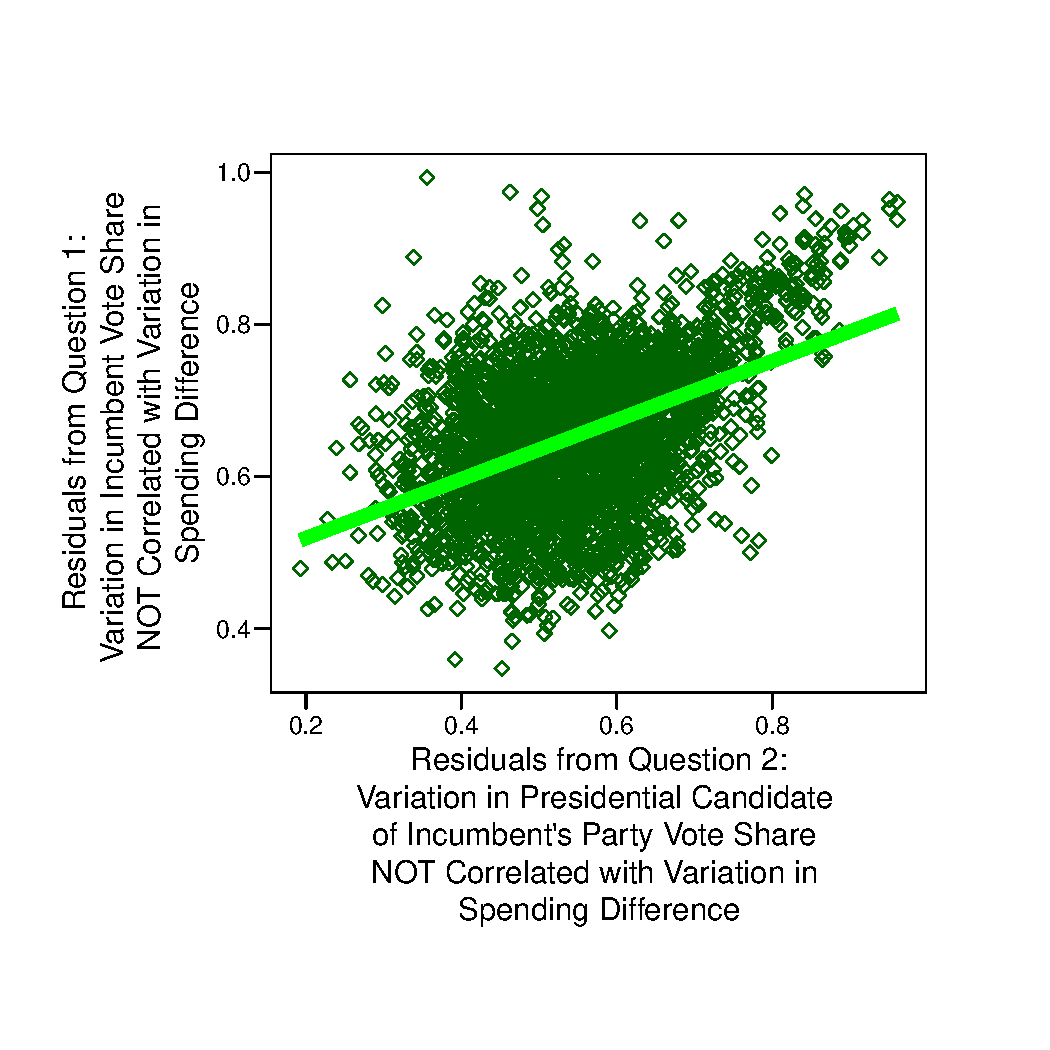
\includegraphics[width=.85\textwidth, trim = 0 2cm 0 2cm, clip]{plot_Q4.pdf}
			\end{figure}

		\item Write the prediction equation.
		
			\texttt Below is the prediction equation for the linear regression where the outcome variable is \texttt{residuals\_diff\_vs\_share} from Question 1 and the explanatory variable is \texttt{residuals\_diff\_vs\_presvote} from Question 2.
			
			\texttt Below is the prediction equation with the relevant values (rounded to two decimal places):
				\begin{align*}
					\text{Predicted "noise" in Q1 Model} = 0 + (0.26 * X_\text{"noise" value from Q2 Model})
				\end{align*}
			
			\texttt One way interpret this equation is that it indicates that larger positive residuals in one model are associated, on average, with positive residuals in the other model - or that the degree of noise in the two models is, on average, systematically dependent.		
		
	\end{enumerate}
	
	\newpage	

\section*{Question 5}
\noindent What if the incumbent's vote share is affected by both the president's popularity and the difference in spending between incumbent and challenger? 
	\begin{enumerate}
		\item Run a regression where the outcome variable is the incumbent's \texttt{voteshare} and the explanatory variables are \texttt{difflog} and \texttt{presvote}.
		
			\lstinputlisting[language=R, firstline=289, lastline=292]{PS3.R}
	
			\begin{table}[!htbp]
				\centering
				\captionsetup{justification=centering, font = footnotesize}
				\caption{Multi-Variate Linear Regression Results} 
				\label{} 
				\begin{tabular}{@{\extracolsep{5pt}}lD{.}{.}{-3} } 
					\\[-1.8ex]\hline 
					\hline \\[-1.8ex] 
					& \multicolumn{1}{c}{\textit{Dependent variable:}} \\ 
					\cline{2-2} 
					\\[-1.8ex] & \multicolumn{1}{c}{voteshare} \\ 
					\hline \\[-1.8ex] 
					difflog & 0.036^{***} \\ 
					& (0.001) \\ 
					& \\ 
					presvote & 0.257^{***} \\ 
					& (0.012) \\ 
					& \\ 
					Constant & 0.449^{***} \\ 
					& (0.006) \\ 
					& \\ 
					\hline \\[-1.8ex] 
					Observations & \multicolumn{1}{c}{3,193} \\ 
					R$^{2}$ & \multicolumn{1}{c}{0.450} \\ 
					Adjusted R$^{2}$ & \multicolumn{1}{c}{0.449} \\ 
					Residual Std. Error & \multicolumn{1}{c}{0.073 (df = 3190)} \\ 
					F Statistic & \multicolumn{1}{c}{1,302.947$^{***}$ (df = 2; 3190)} \\ 
					\hline 
					\hline \\[-1.8ex] 
					\textit{Note:}  & \multicolumn{1}{r}{$^{*}$p$<$0.1; $^{**}$p$<$0.05; $^{***}$p$<$0.01} \\ 
				\end{tabular} 
			\end{table} 
	
			\texttt This multi-variate linear regression model indicates that for \textbf{every 1-unit increase} in the difference in campaign spending between the incumbent and challenger, on average, the vote share for the incumbent increases by \textbf{approx. 0.04 unit points}, controlling for the vote share of the President Candidate of the Incumbent's Party - in other words, 0.04 is the average partial effect of every "unit" of the difference in campaign spending between the incumbent and the challenger on the incumbent's vote share.
			
			Similarly, the average partial effect of every "unit" of the vote share of the Presidential Candidate of the Incumbent's Party on the vote share of the Incumbent is 0.26 (i.e. holding the difference in campaign spending constant).
		
			Each of these partial effects indicate a p-value less than 0.001, which is less than a critical value of 0.05, giving evidence to reject the null hypothesises that the (partial) relationship between the vote share of the Incumbent and both the difference in campaign spending and the vote share of the Incumbent Party's Presidential Candidate is zero - and giving evidence for the alternative hypothesises that each of the relationships is non-zero. It is not possible to indicate a causal relationship with this method.
			
			Further, I note that the $R^2$ value for the multi-variate regression model is 0.45, which is greater than all prior models where the vote share of the incumbent was the outcome variable (Q1 = 0.37; Q3 = 0.21). This indicates that including both explanatory variables informs the model to more accurately estimate the observed data of vote share of the Incumbent official compared to either explanatory variable individually.
			
			Lastly, the F-Statistic has a p-value less than a critical value of 0.05, giving evidence to reject the null hypothesis that these is no relationship between either explanatory variables (vote share of Presidential Candidate of the Incumbent's Party; Difference in Campaign Spending between incumbent and challenger) and the outcome variable (vote share of the incumbent). This also gives evidence to fail to reject the alternative hypothesis that there is a (partial) relationship between at least one explanatory variable and vote share of the Incumbent.
		
		\item Write the prediction equation.
		
			\texttt Below is a generic formal prediction equation for a multi-variate linear regression model:
			
			\begin{align*}
				Y &= \beta_0 + \beta_1 X_1 + \beta_2 X_2 + \ldots + \beta_n X_n + \varepsilon_i
			\end{align*}
			
			\texttt Notice how it is an extension of the bi-variate linear regression The components are:
			\begin{enumerate}
				\item $Y$: The outcome variable
				\item $\beta_0$: The y-intercept (i.e. when the explanatory variable equals zero). When the model includes more than one explanatory variable, $\beta_0$ is the y-intercept with all explanans equal to zero.
				\item $\beta_1, \beta_2, \ldots, \beta_n$: The coefficients. These represent the \textbf{average change} in $Y$ with a one-unit change in the corresponding explanatory variable(s). When the model includes more than one explanatory variable, the coefficients represent the \textbf{partial effect} of each explanan, controlling for all other explanatory variables.
				\item  $X_1, X_2, \ldots, X_n$: The explanatory variable(s).
				\item $\varepsilon_i$: The error (stochastic) term, which represents the unobserved/accounted factors which influence $Y$ yet are not included within the model.
				Note a key assumption for linear regression models is that $\varepsilon_i$ has a constant average effect which cancels out when given a large sample N. This is explained further in previous question.
				
			\end{enumerate}
			
			Inputting the relevant labels and the values for the slopes (coefficients):
			
			\begin{align*}
				\text{Predicted vote share for the incumbent} =\\
				&0.45\\
				&+ (0.04 * X_\text{Difference in Campaign Spending})\\
				&+ (0.26 * X_\text{Vote Share for Presidential Candidate})
			\end{align*}
			
		\item What is it in this output that is identical to the output in Question 4? Why do you think this is the case?
		
			\begin{figure}[H]
				\centering
				\captionsetup{justification=centering, font = footnotesize}
				\caption{Added Variable Plots: Partial Effects\\
					of Difference in Campaign Spending and\\
					of Vote Share of Presidential Candidate\\
					upon Vote Share of the Incumbent.}
				\label{fig:plot_Q5}
				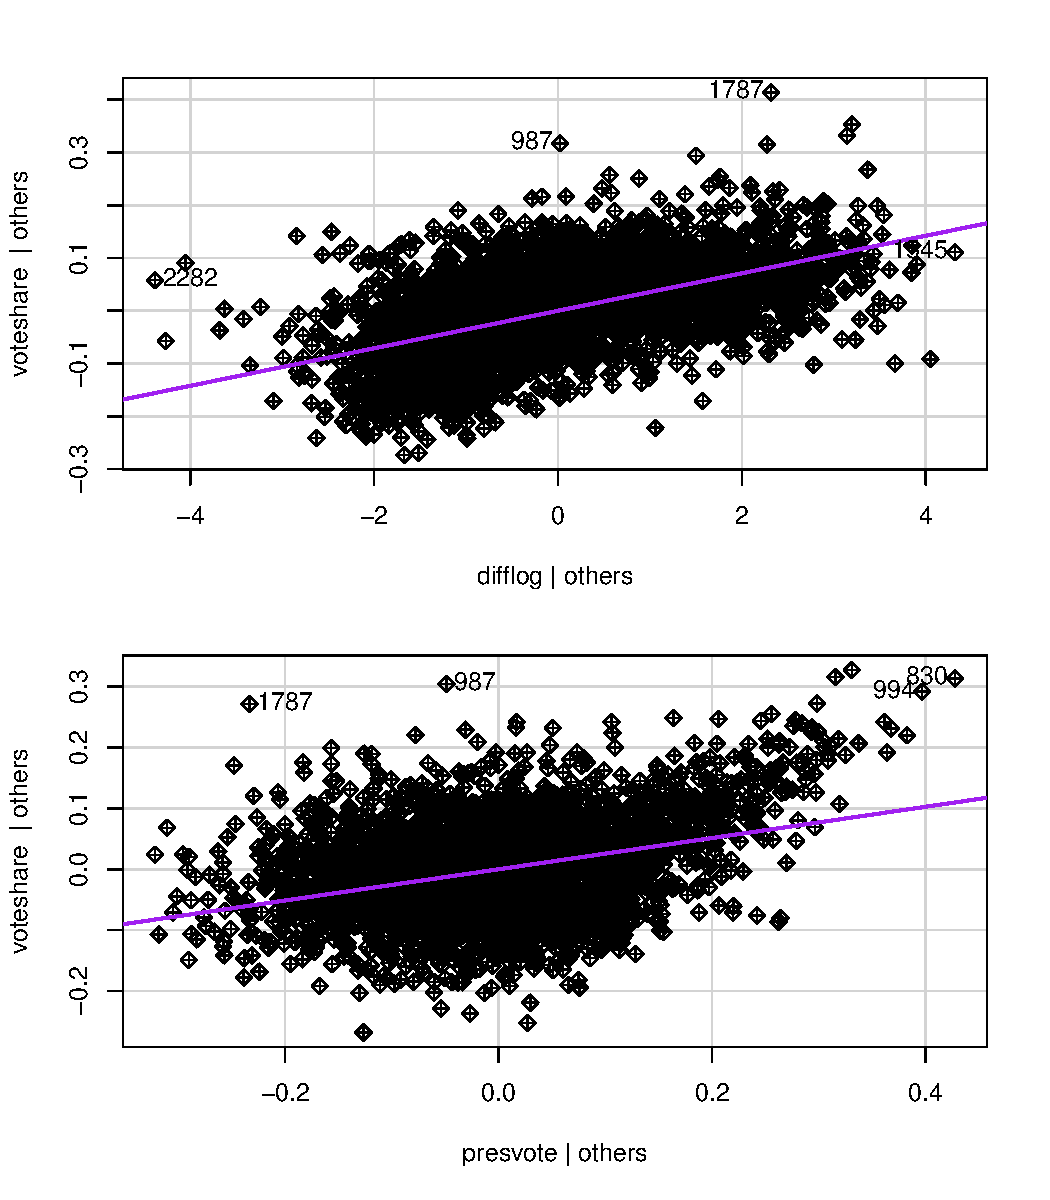
\includegraphics[width=.75\textwidth, clip]{plot_Q5.pdf}
			\end{figure}
			
			\lstinputlisting[language=R, firstline=316, lastline=323]{PS3.R}
			
			\texttt In Table 4, the value of the coefficient for residuals of Q2 Model (predictor = Difference in Campaign Spending, outcome = vote share of the Presidential Candidate) on residuals for Q1 Model (predictor = Difference in Campaign Spending, outcome = vote share of the Incumbent) is \textbf{identical to the partial effect} of the coefficient for vote share of the Presidential Candidate on vote share of the Incumbent in Table 5.
			
			This is because they are measuring the same phenomenon - the y-intercept in Table 4 is effectively 0, indicating that the regression effectively carves out all of the "noise" which the {variation in vote share of the Presidential Candidate} contributes to the {variation in vote share of the Incumbent}. This is the \textbf{partial effect} which is presented in Table 5. This is also demonstrated by how the "Residuals" values for both regressions (the minimum residual value, maximum residual value, median value, etc.) are identical (see R outputs) - these indicate the two regressions are measuring the same data points.
			
			The "Residual Standard Error" in both Table 4 and Table 5 are also identical (with the multi-variate regression including one less degree of freedom as it necessarily uses an additional (\textit{second}) value point in its calculation). This use of additional degree of freedom is also demonstrated in the difference of one between the degrees of freedom value and number of observations used in calculating the F-statistics for the multi-variable regression (two explanatory variables) (Table 5) and bi-variate regression (one explanatory variable) (Table 4).
			
			
		
	\end{enumerate}
	
	


\end{document}
